\documentclass{article}
\usepackage{cite}
\usepackage{graphicx}
\usepackage{hyperref}

\title{Load Balancing Scale-free Graphs on Hybrid Parallel Systems}
\author{Cameron W. Smith}

\begin{document}
\maketitle
\section{Definitions}
\begin{itemize}
  \item data parallel - independently (i.e., without data dependencies) execute
    a single set of instruction on multiple pieces of data concurrently.
    Typically, the instructions are executed by simple, low power, in-order,
    processing units.
  \item task parallel - assign each process in a distributed memory system a
    different set of data and execute a series of instructions sequentially on
    that data.
  \item CPU - a processor composed of hundreds of units that are
    each capable of executing independent instruction sets that interact with
    each other, the filesystem, the network, and the memory hierarchy
    (registers, cache, [high-bandwidth memory,] and main memory).
    Both the task and data parallel programming models can be used for these
    devices~\cite{jeffers2016intel}.
  \item GPU - a processor composed of thousands units in which groups of
    hundreds of units can execute independent instruction sets in lock-step.
    Divergence within the instruction sets caused by conditionals negatively
    impact performance.
    Each unit has access to its local registers, and the device memory.
    The latest generation GPUs now have access to node-memory through hardware-
    and software-based mechanisms.
    The data parallel programming model is used for these devices.
  \item multi-core system - a parallel computer composed of nodes with CPUs
  \item hybrid system - a parallel computer composed of nodes with
    both GPUs and CPUs.
    Each node has at least one GPU per CPU.
  \item Kokkos - APIs for data implementing parallel algorithms that can execute on
    multi-core and GPU systems.  The APIs abstract the implementation details of
    using CUDA, OpenMP, and other data parallel programming
    models~\cite{edwards2013kokkos}.
  \item scale-free graph - a graph with a power-law degree distribution. i.e.,
    the majority graph nodes bound only a few edges (low degree) but some have extremely high
    degree (thousands or millions of bounded edges).
  \item N-Graph - array-based graph data structure that supports multiple edge types
  \item EnGPar - dynamic load balancing and partitioning operations using an N-Graph
\end{itemize}

\section{EnGPar}

The goal of EnGPar is to support multi-criteria, parallel load balancing of
weighted irregular and scale-free graphs.
EnGPar runs on both multi-core and GPU systems from a single code base using
device specific kernels.
The code base provides sufficient graph construction, modification, and
query APIs to support scale-free, graph-based workflows for data mining and
machine learning.
Specific APIs supporting for these workflows enable construction of edge-based
partitions using split nodes (see Figure~\ref{fig:vtxSplitting}).

\section{Challenges}

Constantly evolving massive scale-free graphs, such as those modeling social
networks~\cite{twitter2010,kwak2010twitter}, or the world wide web, require
periodic dynamic load balancing to maintain efficient execution of parallel
discrete event simulations~\cite{carothers2002ross}.
As vertex partitionings of scale-free graphs are known to have low quality
~\cite{abou2006multilevel,lang2004finding,leskovec2009community,pienta2013parallel}
the feasibility of splitting the communication and computation load of high
degree vertices via a split-vertex dynamic partitioning will be evaluated as
part of this research program.
Towards this, the N-Graph interface will be implemented such
that the top few percent of high degree graph vertices, d(u) > εMax(d(u)), are
split and represented by log2(d(u))-1 additional N-Graph vertices and edges, as
depicted in Figure~\ref{fig:vtxSplitting}.
A split-vertex partitioning of the source graph prioritizing the imbalance of
edges over vertices is computed using EnGPar’s multicriteria partitioning
methods.
The graph will then be augmented with additional vertices and edges,
maintaining the original distribution characteristics, and the dynamic
partitioning re-applied.
Support for the design and implementation of scale-free graph operations will be
provided by RPI Professor George Slota.
Professor Slota has extensive experience working on scale-free graphs with over
a trillion edges~\cite{slota_ipdps2017} as a developer of Zoltan2~\cite{zoltan2}, and the
PULP~\cite{slota_ipdps2017} label propagation-based partitioning methods.

\begin{figure}
  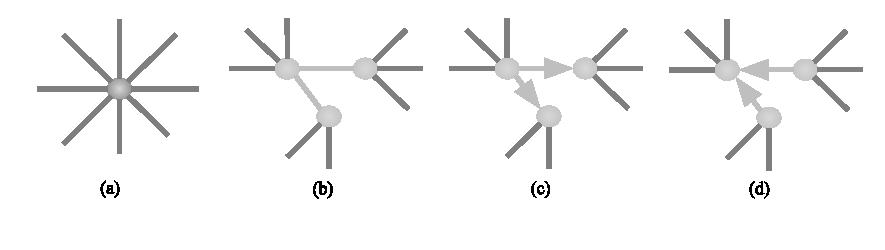
\includegraphics[width=\textwidth]{../ngraph/vtxSplitting.eps}
  \caption{\label{fig:vtxSplitting}
    High degree vertex splitting. 
    The original high degree vertex in (a), the split N-graph representation in
    (b), and the scatter and gather update protocol in (c) and (d) respectively.
  }
\end{figure}

The quality of the partitionings will be evaluated by executing the massively
parallel ROSS~\cite{carothers2002ross,mubarak2012modeling,barnes2013warp}
open-source discrete event simulation engine.
Through on-going collaborations with RPI Professor Chris Carothers, the principal
author of ROSS, a message passing based shared state update of split vertices
using a scatter/gather update
protocol~\cite{gonzalez2012powergraph,sahni2009scalable} as depicted in
Figure~\ref{fig:vtxSplitting} will be integrated into ROSS.

The key challenge to implementing EnGPar is quickly partitioning massive
scale-free graphs for workflows executing on both GPU and multi-core systems.
Critial to efficient execution is the use of operations that apply to graph
nodes or edges concurrently (via vectorization of parallel loop constructs).
Critically, users must implement their procedures without branching (i.e.,
{\texttt if} statements) or loop inter-dependencies
(i.e., a given iteration of the loop must be able to execute independently of
all other iterations).
Thus, we will be develop APIs to minimize the burden on users accustomed to
serial, iterator-based graph interactions.

One specific challenge will be maintaing efficiency when graph queries or
modification procedures involve only a small subset of the domain.
For example, during a breadth first traveral the front size significantly limits
concurrency.
Thus, using low overhead cache-coherency mechanisms, we will dynamically
relocate the execution of kernels from the CPU, which excels at high speed
serial computation, to the GPU when concurrency becomes sufficient.
Ideally, this careful matching of algorithm concurrency to processing resources
will reduce overheads caused by the forced use of GPUs for near-serial
operations, and/or development time spent implementing complex algorithms to
force a procedure to execute on a GPU.

\section{Approach}

For both CPU and GPU data parallel algorithms Kokkos~\cite{edwards2013kokkos}
will be used to implement user-facing EnGPar APIs that support operation on
large groups of mesh entities.
User APIs to query (i.e., read only) single mesh entities will use the
array-based structures to perform atomic look ups.

\section{Questions}
\begin{itemize}
  \item What is the overhead for using the cache coherency between the
    CPU and the GPU?
    The current systems don't support this advanced feature of NVLink so we will
    likely have to wait another year to find out.
\end{itemize}

\bibliographystyle{scorec-refs/IEEEtran_rpi}
\bibliography{scorec-refs/scorec-refs}

\end{document}
